\documentclass[12pt]{article}
\usepackage[utf8]{inputenc}
\usepackage{amsmath}
\usepackage{graphicx}
\usepackage{array}
\usepackage{geometry}
\geometry{margin=2.5cm}
\usepackage{titlesec}
\usepackage{float}
\usepackage{grffile} % importante para nombres de archivo con puntos o caracteres especiales
\titleformat{\section}{\centering\bfseries\uppercase}{\thesection}{1em}{}

\begin{document}

\section*{ DISEÑO A FLEXIÓN DE VIGA 30X50 }

\begin{minipage}[t]{0.48\textwidth}
\begin{tabular}{|l|c|}
\hline
Base (b) & 30.00 cm cm \\
Altura (h) & 50.00 cm cm \\
Recubrimiento (r) & 4.00 cm cm \\
Estribo (\ensuremath{\phi_e}) & 0.95 cm cm \\
Varilla principal (\ensuremath{\phi_s}) & 1.59 cm cm \\
f'c & 210.00 kgf/cm² kgf/cm$^2$ \\
fy & 4200.00 kgf/cm² kgf/cm$^2$ \\
\hline
\end{tabular}
\end{minipage}
\hfill
\begin{minipage}[t]{0.48\textwidth}

\begin{figure}[H]
\centering
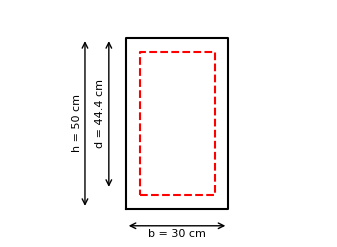
\includegraphics[height=5cm]{ section.png }
\end{figure}

\end{minipage}

\vspace{0.5cm}





\vspace{0.5cm}





\vspace{0.5cm}





\vspace{0.5cm}





\vspace{0.5cm}





\vspace{0.5cm}





\vspace{0.5cm}





\end{document}